\documentclass{article}

% if you need to pass options to natbib, use, e.g.:
%     \PassOptionsToPackage{numbers, compress}{natbib}
% before loading neurips_2018

% ready for submission
% \usepackage{neurips_2018}

% to compile a preprint version, e.g., for submission to arXiv, add add the
% [preprint] option:
%     \usepackage[preprint]{neurips_2018}

% to compile a camera-ready version, add the [final] option, e.g.:
\usepackage[final]{nips_2018}

% to avoid loading the natbib package, add option nonatbib:
%     \usepackage[nonatbib]{neurips_2018}

\usepackage[utf8]{inputenc} % allow utf-8 input
\usepackage[T1]{fontenc}    % use 8-bit T1 fonts
\usepackage{hyperref}       % hyperlinks
\usepackage{url}            % simple URL typesetting
\usepackage{booktabs}       % professional-quality tables
\usepackage{amsfonts}       % blackboard math symbols
\usepackage{nicefrac}       % compact symbols for 1/2, etc.
\usepackage{microtype}      % microtypography
\usepackage{amsmath}
\usepackage{algorithm,algorithmic}
\usepackage{graphicx}


\newcommand{\fracpartial}[2]{\frac{\partial #1}{\partial  #2}}
\newcommand{\Dir}[0]{\textrm{Dirichlet}}
\newcommand{\Ray}[0]{\textrm{Rayleigh}}
\newcommand{\gam}[0]{\textrm{Gamma}}
\newcommand{\dgamma}[0]{\textrm{Gamma}}
\newcommand{\dpoisson}[0]{\textrm{Poisson}}
\newcommand{\dbeta}[0]{\textrm{Beta}}
\newcommand{\dbern}[0]{\textrm{Bernoulli}}
\newcommand{\dunif}[0]{\mathrm{Uniform}}
\newcommand{\dgig}[0]{\textrm{GIG}}
\newcommand{\dnormal}[0]{\mathrm{Normal}}
\newcommand{\dt}[0]{\mathrm{t}}
\newcommand{\igamma}[0]{\textrm{Gamma}^{-1}}
\newcommand{\rayl}[0]{\textrm{Rayleigh}}
\newcommand{\Exp}[0]{\textrm{Exponential}}
\newcommand{\Bet}[0]{\textrm{Beta}}
\newcommand{\GEM}[0]{\textrm{GEM}}
\newcommand{\DP}[0]{\textrm{DP}}
\newcommand{\ESS}[0]{\mathrm{ESS}}
\newcommand{\bm}[1]{\boldsymbol{#1}}
\newcommand{\bbeta}{\bm{\beta}}
\newcommand{\bpi}{\bm{\pi}}
\newcommand{\bomega}{\bm{\omega}}
\newcommand{\bgamma}{\bm{\gamma}}
\newcommand{\blambda}{\bm{\lambda}}
\newcommand{\bphi}{\bm{\phi}}
\newcommand{\btheta}{\bm{\theta}}
\newcommand{\bmu}{\bm{\mu}}
\newcommand{\bb}{\bm{b}}
\newcommand{\bk}{\bm{k}}
\newcommand{\bl}{\bm{l}}
\newcommand{\bn}{\bm{n}}
\newcommand{\bw}{\bm{w}}
\newcommand{\bz}{\bm{z}}
\newcommand{\bx}{\bm{x}}
\newcommand{\bX}{\bm{X}}
\newcommand{\by}{\bm{y}}
\newcommand{\bZ}{\bm{Z}}
\newcommand{\bW}{\bm{W}}
\newcommand{\bS}{\bm{S}}
\newcommand{\bH}{\bm{H}}
\newcommand{\Mult}{\textrm{Multinomial}}
\newcommand{\N}{\mathcal{N}}
\newcommand{\NEW}{\textrm{\tiny new}}
\newcommand{\OLD}{\textrm{\tiny old}}
\newcommand{\sigmat}{\sigma^2}
\newcommand{\IBP}{\textrm{IBP}}
\newcommand{\E}{\mathbb{E}}
\newcommand{\V}{\mathbb{V}}
\newcommand{\Eq}{\mathbb{E}_q}
\newcommand{\cL}{\mathcal{L}}
\newcommand{\cB}{\mathcal{B}}
\newcommand{\cC}{\mathcal{C}}
\newcommand{\cV}{\mathcal{V}}
\newcommand{\cHq}{\mathcal{H}_q}
\newcommand{\test}[1]{\mbox{$#1$}^{\small \mbox{test}}}
\newcommand{\alphaW}{\alpha^{(W)}}
\newcommand{\alphaH}{\alpha^{(H)}}
\newcommand{\betaW}{\beta^{(W)}}
\newcommand{\betaH}{\beta^{(H)}}
\newcommand{\gammaW}{\gamma^{(W)}}
\newcommand{\gammaH}{\gamma^{(H)}}
\newcommand{\gammaT}{\gamma^{(\theta)}}
\newcommand{\rhoW}{\rho^{(W)}}
\newcommand{\rhoH}{\rho^{(H)}}
\newcommand{\rhoT}{\rho^{(\theta)}}
\newcommand{\tauW}{\tau^{(W)}}
\newcommand{\tauH}{\tau^{(H)}}
\newcommand{\tauT}{\tau^{(\theta)}}
\newcommand{\muW}{\hat{W}}
\newcommand{\muH}{\hat{H}}
\newcommand{\Var}{\textrm{Var}}
\newcommand{\LF}{\mathrm{Leapfrog}}

\title{MCMC convergence diagnostics with uncertainty using gradient-boosted machines}

% The \author macro works with any number of authors. There are two commands
% used to separate the names and addresses of multiple authors: \And and \AND.
%
% Using \And between authors leaves it to LaTeX to determine where to break the
% lines. Using \AND forces a line break at that point. So, if LaTeX puts 3 of 4
% authors names on the first line, and the last on the second line, try using
% \AND instead of \And before the third author name.

\author{%
	 Ben Lambert\\
	 MRC Centre for Global Infectious Disease Analysis\\
	 School of Public Health\\
	 Imperial College London\\
	 W2 1PG, United Kingdom\\
	 \texttt{ben.c.lambert@gmail.com} \\
}

\begin{document}
% \nipsfinalcopy is no longer used

\maketitle

\begin{abstract}
	Markov chain Monte Carlo (MCMC) has transformed inference of Bayesian models over the past three decades: mainly because of this, Bayesian inference is now a workhorse of applied scientists. Despite its importance, MCMC is a notoriously subtle beast. Indeed, the words of statisticians often echo that MCMC "should be used with caution, almost as a last resort"; the problem is that we are usually at the "last resort" for interesting models. Central to these concerns is the difficulty in determining whether Markov chains have converged to the posterior distribution. Under general conditions, MCMC sampling will converge asymptotically to the posterior distribution, but this makes no guarantees about its finite sample performance. The predominant method for monitoring convergence is to run multiple chains and monitor individual chains' characteristics and compare these to the population of chains as a whole: if the within-chain and between-chain summaries are comparable, then this may indicate that the chains have converged to a stationary distribution. Collectively, these summary statistics aim to determine whether or not it is possible to determine the chain that generated a particular sample: if you can, then the chains have not mixed and convergence has not occurred. Here, we introduce a new method for probing convergence based on training machine learning algorithms to classify samples according to the chain that generated them. A benefit of this approach is that it provides a single statistic across all parameters that captures whether convergence has occurred, although individual variables' importance for this metric can also be determined. Additionally, this measure of convergence is not based on any single characteristic of the sampling distribution (for example, the mean, as for the predominant $\hat{R}$); instead using all the information in the chain. The method is straightforward to implement and could be an additional check on convergence for applied analyses.
\end{abstract}

\section{Introduction}

Chris Holmes quote reference.

Can we determine uncertainty in convergence?

\section{Method}

\section{Results}
To illustrate the utility of our approach, we use examples taken from \cite{vehtari2019rank}.

\subsection{Heterogeneity in chain variance}\label{sec:heterogeneity}
We generate four Markov chains, where each samples from an autoregressive order 1 (AR1) process of the form,
%
\begin{equation}
X_t = \rho X_{t-1} + \epsilon_t
\end{equation}
%
where $\epsilon_t\stackrel{i.i.d.}{\sim}\mathcal{N}(0, \sigma)$. Three of the chains share the same $\sigma=\bar{\sigma}$, whereas the other chain has $\sigma=1/3\bar{\sigma}$, so that it has $1/3$ of the (unconditional) variance of the others. In each replicate, we simulate 1000 iterations from all four chains and fit a gradient-boosted model to a labelled training set of 2800 randomly-chosen samples, and use it to classify samples according to the chain which generated them in an independent test set comprising the remaining 1200 observations. We perform 1000 replicates and, in each case, we report the ratio of accuracy of the predictions to the null model which assigns observations to chains uniformly at random (i.e. having an accuracy of 25\%).

In Fig. \ref{fig:ar1}A, we show how an example model fit to training data classifies observations by chain according to the sample's value. Unsurprisingly, since the fourth chain has a smaller variance, observations close to zero are likely to be classified as being generated by this chain. In Fig. \ref{fig:ar1}B, we show that the accuracy ratio is well above 1 for all replicates.

\begin{figure}[h]
	\centerline{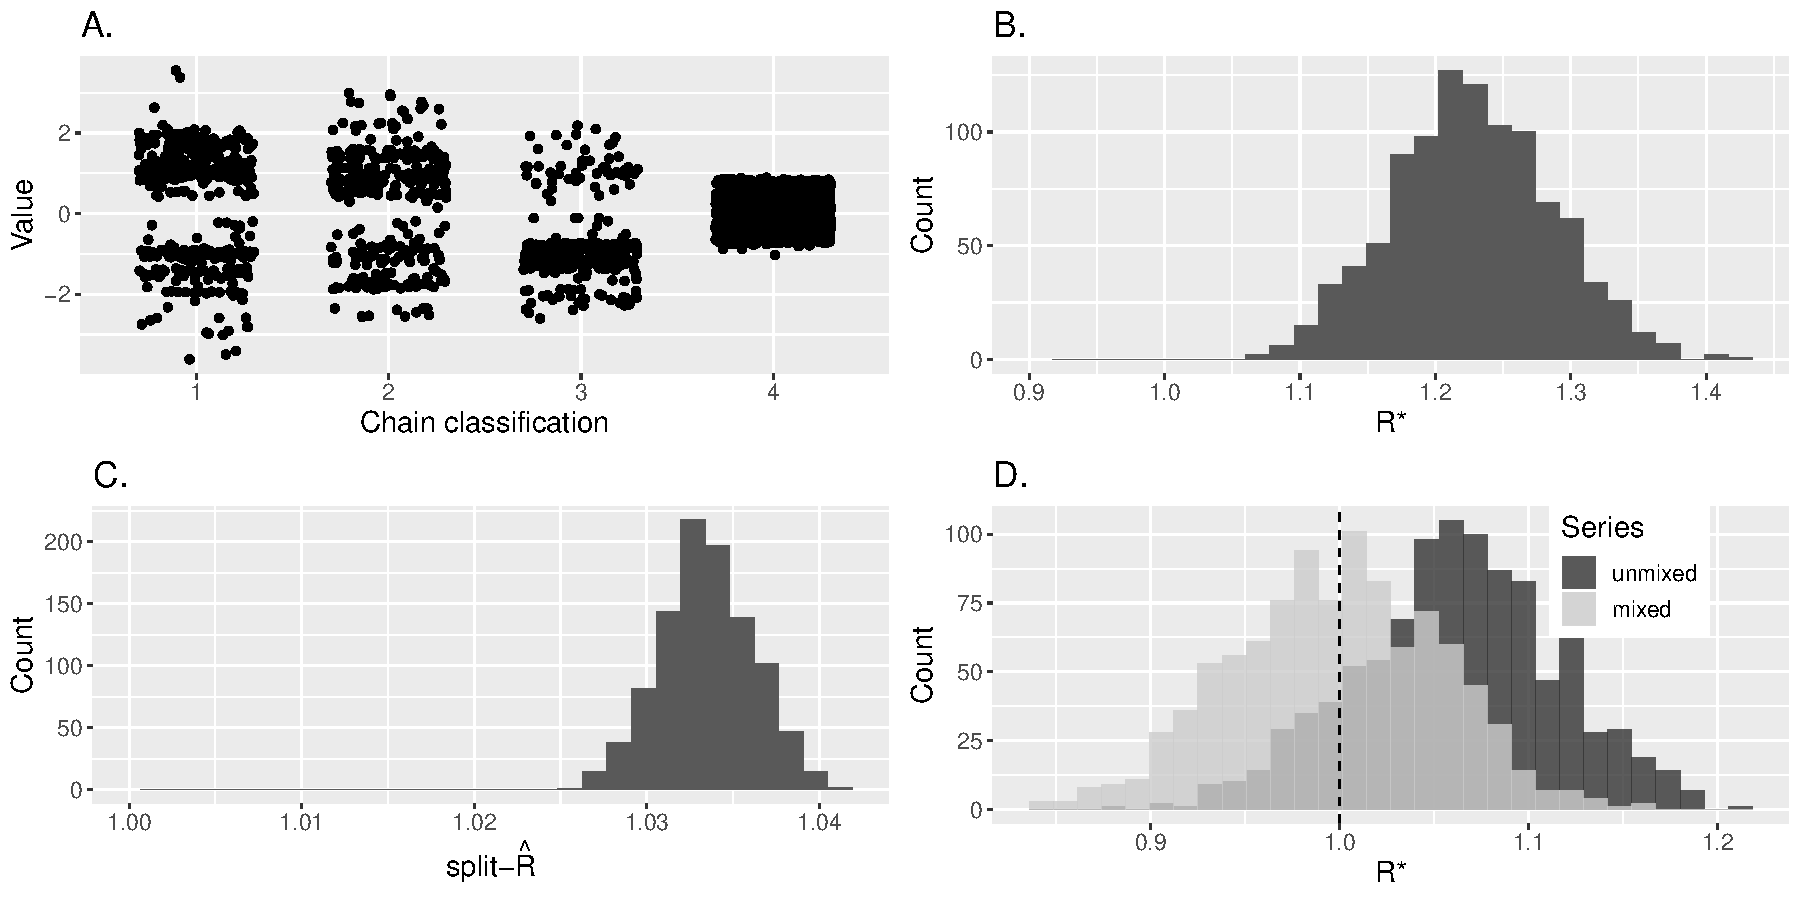
\includegraphics[width=1.0\textwidth]{../output/ar1.pdf}}
	\caption{\textbf{Autoregressive example.} A shows how the gradient-boosted model's classifications vary according to the sample's value for an example model fit; B shows the ratio of predictive accuracy to the null model accuracy across 1000 replicates; C shows the uncertainty in accuracy ratio for two series described in the text. See the R markdown file in the SOM for hyperparameters and code for fitting the gradient-boosted model.}
	\label{fig:ar1}
\end{figure}

Since the gradient-boosted models return a probability simplex for each sample, which indicates the probability it was generated by each chain, we are also able to generate uncertainty in our measure of convergence. For each sample, we randomly sample a chain classification from a multinomial distribution with class probabilities given by the outputs from the machine learning model then check whether this matches the true chain identity. The accuracy is then given by the percentage of samples where the prediction is correct. By repeating this exercise across a number of replicates, we obtain an uncertainty in the accuracy, which we convert to an accuracy ratio as before.

We demonstrate this idea using two datasets: one generated as described above, where one chain (out of four) has a lower variance than the others (we call this the "unconverged data"); and another, where all chains sample from the same distribution (we call this the "converged data"). In Fig. \ref{fig:ar1}C, we show the uncertainty distributions for the accuracy ratio that result from sampling from the underlying fit of a single gradient-boosted model to each dataset. For the unconverged data, the distribution has its bulk of mass away from 1, indicating lack of convergence. For the converged data, the distribution is centred on 1, indicating convergence. 

\subsection{Infinite chain variance}
Use Cauchy example

\subsection{Hierarchical model: Eight schools}
In this example, we examine a simple classic example used to highlight difficulties in performing sampling for hierarchical models: referred to as the "Eight schools" model (see Section 5.5 in \cite{gelman2013bayesian}), which aimed to determine the effects of coaching on SAT scores in eight schools. 

The model can be parameterised two ways, as described in \cite{vehtari2019rank}. The simplest way is referred to as the "centered" parameterisation and exactly mirrors the underlying statistical model,
%
\begin{align*}
\theta_j &\sim \N(\mu, \tau) \\
y_j &\sim \N(\theta_j, \sigma_j).
\end{align*}
%
The non-centered parameterisation recodes this model in a way which does not affect the joint distribution of $(\tilde{\theta}, \mu, \tau, \sigma)$ but makes it easier to sample from it, by introducing auxillary variables. This can be written as,
%
\begin{align*}
\tilde{\theta}_j &\sim \N(0, 1) \\
\theta_j &= \mu + \tau \tilde{\theta}_j \\
y_j &\sim \N(\theta_j, \sigma_j).
\end{align*}
%
In both cases, $\theta_j$ are the treatment effects in the eight schools, and $\mu, \tau$ represent the population mean and standard deviation 
of the distribution of these effects. In the centered parameterization, the $\theta$ are parameters, whereas in the non-centered parameterization, the $\tilde{\theta}$ are parameters and $\theta$ is a derived quantity.

We first used Stan \cite{carpenter2017stan} to sample from the centered model using 4 chains. Like \cite{vehtari2019rank}, we use settings that reduce the chance of divergent iterations for the NUTS algorithm \cite{hoffman2014no}, meaning that the resultant sampling distribution is likely to be biased. We also used Stan with the same algorithm settings to sample from the non-centered model.

To see how $R^*$ performed on this example, we first split each of the (post-warm-up) chains in two, as is done by default in Stan \cite{carpenter2017stan} and in \cite{vehtari2019rank}, resulting in 500 iterations across 8 chains. Next, we trained the gradient-boosted model on a training set comprising 2800 samples, and used it to classify the causative chain for 1200 independent test samples. Following the same approach as in \S\ref{sec:heterogeneity}, we generated uncertainty in $R^*$ for both the centered and non-centered models. The resultant distributions for $R^*$ are shown in Fig.\ref{fig:eight_schools}A. In this plot, it is clear that whereas the centered model shows signs of convergence, the non-centered model does not: intuitively, the chains have not sufficiently mixed with themselves nor the others meaning that the causative chain can be predicted with reasonable accuracy from the sample location.

In gradient-boosted tree models (GBMs), it is possible to calculate variable importance (see, for example, \cite{friedman2001greedy} and \cite{greenwell2019package}), and this allows us to determine which variables were mostly responsible for predictive power. For GBM fitted to the centered model, the most important variable was $\tau$, followed by Stan's $lp$ variable (we also include this in our training and testing data), followed by $\mu$ and $\theta_2$. Interestingly, these were slightly differently ordered according to Stan's $\hat{R}$, with $lp$ having the highest value ($\hat R = 1.06$), followed by $\tau$ ($\hat R = 1.02$), then a host of variables with ($\hat R = 1.01$).

In addition, to illustrate the power of $R^*$, we also repeat the analysis but, this time, do not split the chains in two. The results are shown in Fig.\ref{fig:eight_schools}B. In this case, because the unsplit chains do not mix with themselves, it is harder to accurately predict the chain that generated each sample, meaning that the centered model $R^*$ values are shifted leftwards. Despite this, however, the distribution for $R^*$ still does not strongly overlap with $R^*=1$, indicating that the model has not converged.

\begin{figure}[h]
	\centerline{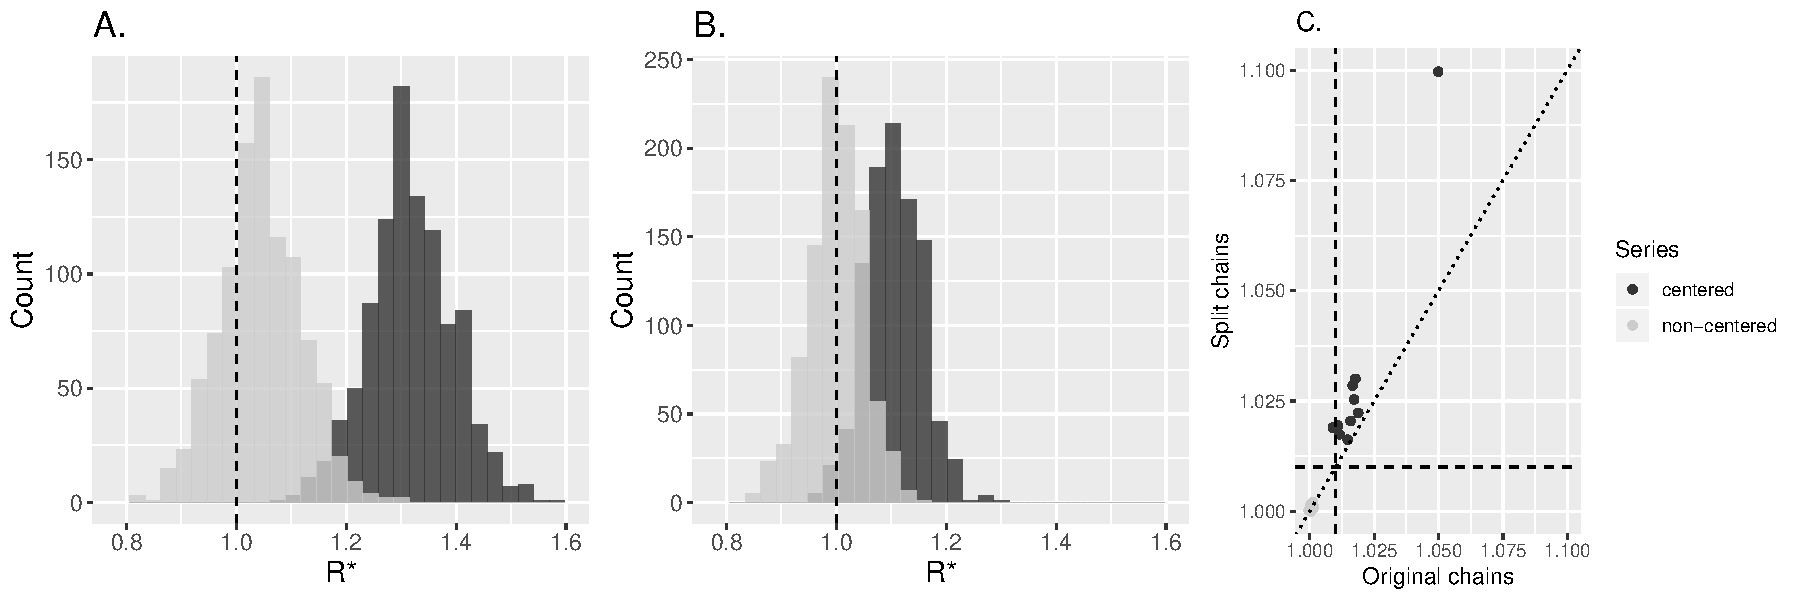
\includegraphics[width=1.0\textwidth]{../output/eight_schools.pdf}}
	\caption{\textbf{Eight schools example.} A shows samples from the $R^*$ distribution when splitting chains; B shows the same but using the 4 original chains. In both cases, the plots show 1000 samples. See the R markdown file in the SOM for hyperparameters and code for fitting the gradient-boosted model.}
	\label{fig:eight_schools}
\end{figure}

\section{Discussion}
Add in index variable into set of predictors.
Relative insensitivity of GBM to settings (in all examples we used the same hyperparameters)



	
\bibliographystyle{unsrt}
\bibliography{bibliography} 
	
\end{document}
